\documentclass[%
    a4paper, twoside, dissertation, fontsize=12pt%
]{tufte-book}
\hypersetup{colorlinks}

%%%%%%%%%%%%%%%%%%%%%%%%%%%%%%%%%%%%%%%%%%%%%%%%%%%%%%%%%%%%%%%%%%%%%%%%%%%%%%%
%% Metadata
\title{data-driven precision cardiology}
\author[Peter Christoffer Holm]{Peter Christoffer Holm}
\publisher{University of Copenhagen}
%%%%%%%%%%%%%%%%%%%%%%%%%%%%%%%%%%%%%%%%%%%%%%%%%%%%%%%%%%%%%%%%%%%%%%%%%%%%%%%

\usepackage{microtype}
\usepackage{booktabs}
\usepackage{lipsum}
\usepackage{pdfpages}
\usepackage{blindtext}
\usepackage{appendix}

% For graphics / images
\usepackage{graphicx}
\setkeys{Gin}{width=\linewidth,totalheight=\textheight,keepaspectratio}
\graphicspath{{graphics/}}

% The fancyvrb package lets us customize the formatting of verbatim
% environments.  We use a slightly smaller font.
\usepackage{fancyvrb}
\fvset{fontsize=\normalsize}

% Hanging parentheses and asterisks
\newcommand{\hangp}[1]{\makebox[0pt][r]{(}#1\makebox[0pt][l]{)}}
\newcommand{\hangstar}{\makebox[0pt][l]{*}}

% Prints the month name (e.g., January) and the year (e.g., 2008)
\newcommand{\monthyear}{%
  \ifcase\month\or January\or February\or March\or April\or May\or June\or
  July\or August\or September\or October\or November\or
  December\fi\space\number\year
}

% Custom macros
\newcommand{\na}{\quad--}
\newcommand{\blankpage}{\newpage\hbox{}\thispagestyle{empty}\newpage}

%%%%%%%%%%%%%%%%%%%%%%%%%%%%%%%%%%%%%%%%%%%%%%%%%%%%%%%%%%%%%%%%%%%%%%%%%%%%%%%

\begin{document}
\frontmatter
\maketitle

\begin{@empty}
~\vfill
\thispagestyle{empty}
\setlength{\parindent}{0pt}
\setlength{\parskip}{\baselineskip}

\smallcaps{Candidate}

\textbf{Peter Christoffer Holm}, MSc

Novo Nordisk Foundation Center for Protein Research,
University of Copenhagen, Denmark

\smallcaps{Supervisors}

\textbf{Søren Brunak}, PhD, Professor 
(principal supervisor)

Novo Nordisk Foundation Center for Protein Research, 
University of Copenhagen, Denmark

\textbf{Henning Bundgaard}, PhD, Dr.Med, Professor 
(co-supervisor)

Department of Cardiology,
Copenhagen University Hospital, Denmark

\textbf{Karina Banasik}, PhD, Associate Professor 
(co-supervisor)

Novo Nordisk Foundation Center for Protein Research, 
University of Copenhagen, Denmark

\vspace{2em}

\par\smallcaps{Published by the \thanklesspublisher}

\vspace{5em}

\par This document was created using the \LaTeX{} typesetting software.
The layout is based on the \texttt{tufte-latex} document class,
and the main body of the text is set in \textsf{ETbb} and \textsf{Libertine}.
Unless otherwise indicated, all figures and graphics in the main text
are either the property of the author or are in the public domain.

%\par\textit{First printed, \monthyear}

Copyright \copyright\ \the\year\ \thanklessauthor
\end{@empty}

\cleardoublepage
 
\tableofcontents
\listoffigures
\listoftables
\cleardoublepage

%%%%%%%%%%%%%%%%%%%%%%%%%%%%%%%%%%%%%%%%%%%%%%%%%%%%%%%%%%%%%%%%%%%%%%%%%%%%%%%

\mainmatter

\chapter{Introduction}
\section{Survival analysis}

\Blindtext[2]
\Blindtext[2]

\section{Machine Learning}

\Blindtext[5]

%%%%%%%%%%%%%%%%%%%%%%%%%%%%%%%%%%%%%%%%%%%%%%%%%%%%%%%%%%%%%%%%%%%%%%%%%%%%%%%

\backmatter
% \bibliography{sample-handout}
% \bibliographystyle{plainnat}

%%%%%%%%%%%%%%%%%%%%%%%%%%%%%%%%%%%%%%%%%%%%%%%%%%%%%%%%%%%%%%%%%%%%%%%%%%%%%%%

\part*{Appendix}

\appendix

\chapter{Paper 1}

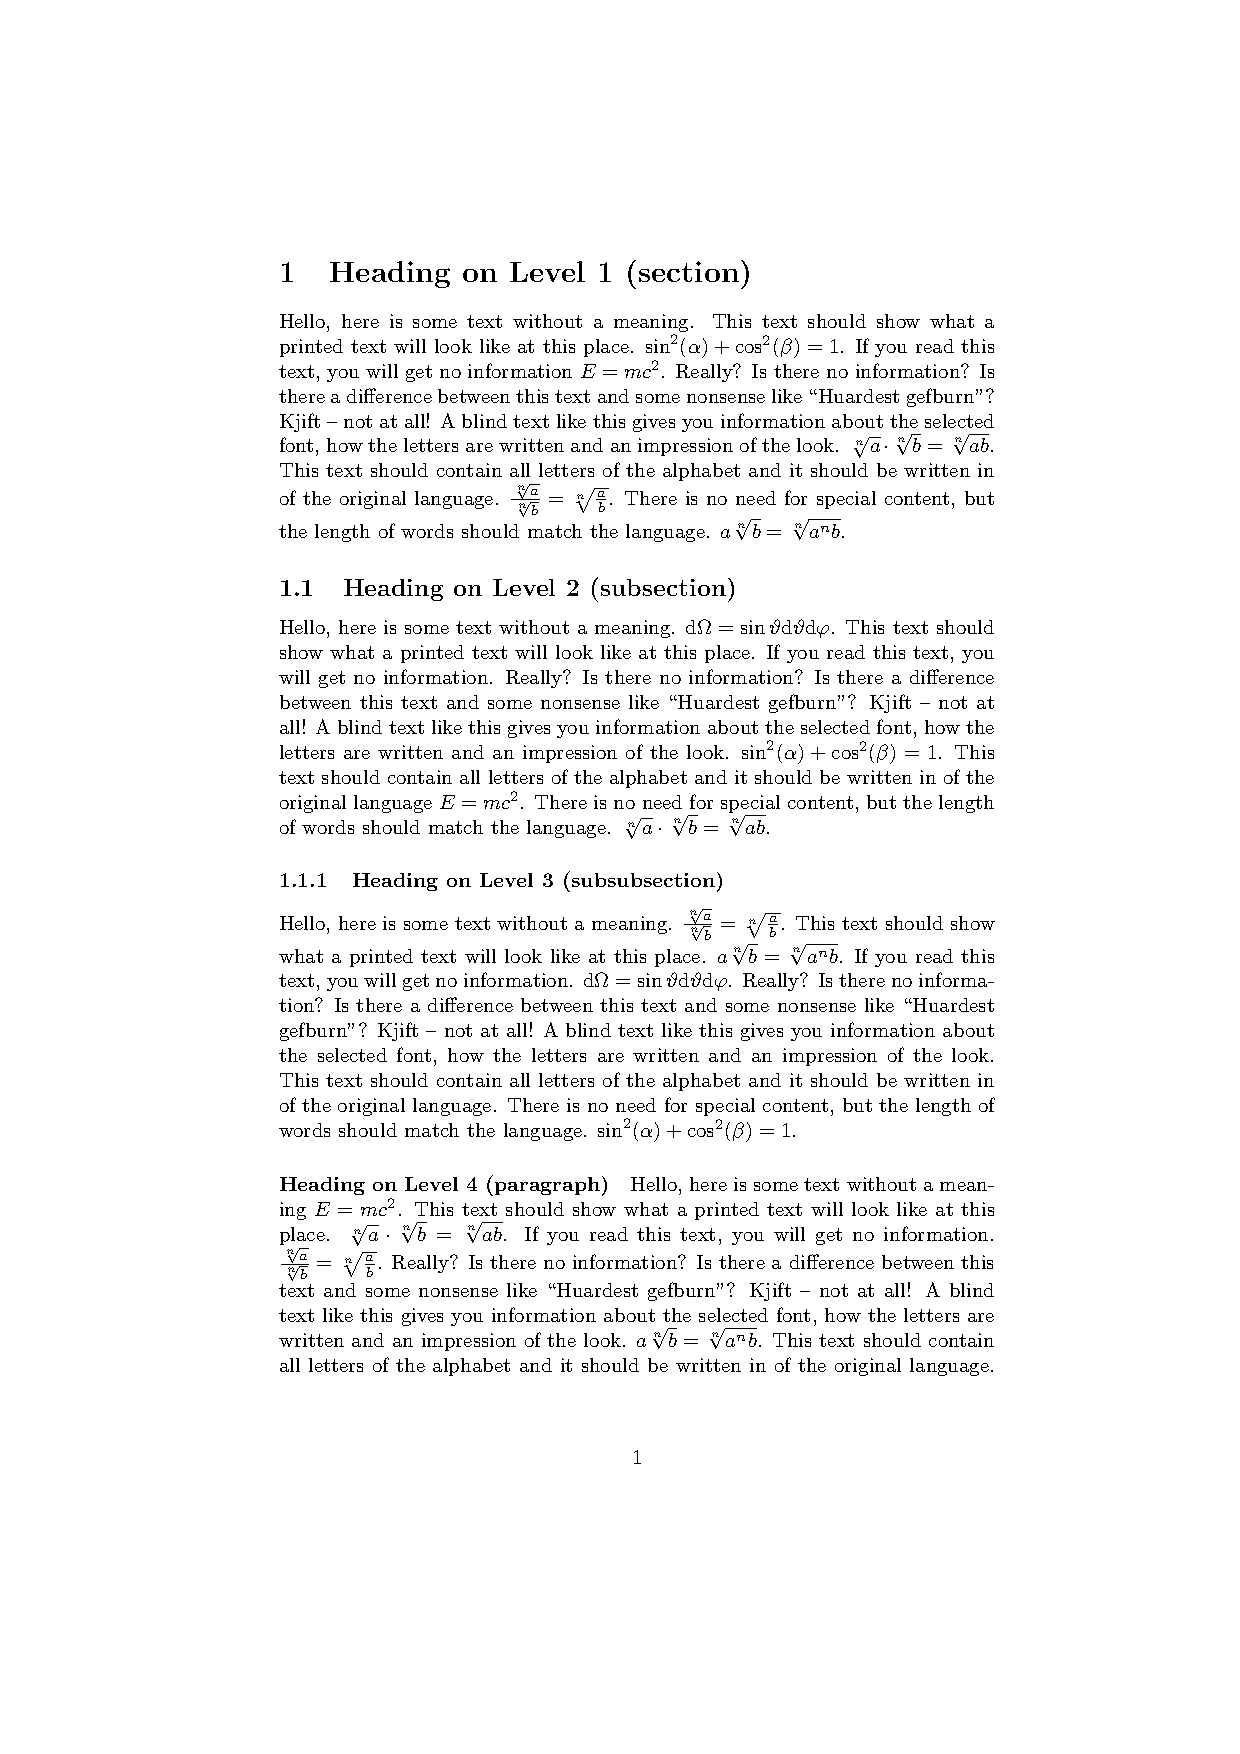
\includepdf[%
    frame=true, scale=0.8, pages=-, pagecommand={}%
]{assets/dummy.pdf}

\end{document}
